% main.tex, to be used with thesis.tex
% This contains the main work of your thesis.

%\bibliography{thesis}  % uses the references stored in Chapter1Radar.bib

\chapter{Experimental Results: Correct Behavior and Performance}

As discussed in the previous chapter, the implementation of a data persistence
layer for NetBEAMS followed the requirements defined in chapter 4 having in
mind the classification of the SF-BEAMS sensor network and the software
infrastructure provided by the Data Sensor Platform. As a result, the
implementation was developed using the infrastructure provided by the online
version-control system repository from NetBEAMS, whose documentation is
detailed in section \ref{sec:dsp-data-persistence-implementation}.

First, this chapter details the experiment setup designed to evaluate the
proposed implementation, showing the measurement results collected from the
simulation log and based on the user experience while reusing the collected
data. Last, but not least, the pertinent discussion of this work is devided up
into different sections, each of them analyzing different aspects related to
data persistence for NetBEAMS, amongo others.

\section{Experiment Setup}

The experiment was designed to support different scenarios of a regular use of
the mongoDB system infrastructure, simulating the activities of data collection
from the SF-BEAMS network using the NetBEAMS infrastructure. First, the setup
for the data collection of randomly generated data was implemented, which
directly uses NetBEAMS already existing classes. Then, the implementation of
the CRUD scenarios were implemented in different programming languages, from
the data insertion scenario using the Java Programming Language, and then the
remaining operations using the Javascript Scripting language \cite{javascript}
and the Python Programming Language \cite{python}. Similarly, an open-source web
application, developed in the Ruby Programming language \cite{ruby}, was also
used. The experiment scripts were writen using Shell Bash Script Language
\cite{bashshell} and is responsible for orchestrasting the execution of one
single experiment ``run''.

\subsection{Experiments Artifacts}

Different artifacts were created to perform the different experiments
operations. The Create function was developed in Java, without the interversion
of the DSP or OSGi, isolating only the functionalities of provided by CRUD
service class DSPMongoCRUDService (Listing \ref{file:dsp-mongo-service}),
responsible for the connection handling with mongoDB, as well as the insertion
operation from NetBEAMS. As described in section \ref{sec:dsp-details}, the
current version of NetBEAMS supports the data collection for the YSI Sonde
device, among others used for demo purposes such as a software sensor that
captures the mouse activities over a window. The documentation of both data
types is seen in section \ref{sec:dsp-payload-implementation}. In this way, the
DSP Data Persistence, as described in the previous section, supports both data
types to be persisted.

In order to exercise mongoDB with the same data collected from NetBEAMS, the
existing Java class TestSondeData (Listing
\ref{file:random-ysi-data-generator}), was refactored to provide a random
instance generator for the YSI Data handler implemented in the Java class
SondeDataType (Listing \ref{file:main-ysi-data-handler}). When the Insert
function is executed, the created instances are transferred from the JVM to
the mongoDB, and stored in the collection ``SondeDataContainer''. Specific
details about the execution of mongoDB are depicted in section
\ref{sec:mongodb-deployment}. Finally, the implementation of the experiment
in the Java class DSPMessageToMongoDBExperiment (Listing
\ref{file:experiment-dsp-java-executor}) was responsible for managing the
creation and insertion of any workload composed by instances of the class
SondeDataType in a bulk manner.

Similarly, the support for the Retrieve, Update and Delete operations against
the inserted workload were implemented using Javascript, as shown in Listing
\ref{file:experiment-scenarios}, respectively by the function calls ``find'',
``update'' and ``remove'' over the collection ``SondeDataContainer''.
Similarly, in order to implement a customizable export system that converts
from mongoDB into the format OpenDAP, a simpler prototype script was developed
in Python, as shown in Listing \ref{file:experiment-export-python}. As a result
of the execution of this script, the exported artifact has the same format as
described in Listing \ref{file:rtc-ysi-opendap}. 

On the other hand, the execution of the main experiment shell script requires
the use to provide the size of the workload, as shown in listing
\ref{cmd:run-persistence-experiment}.

\lstset{label=cmd:run-persistence-experiment,caption=Running main experiment
shell script}
\begin{lstlisting}
marcello@netbeams-dev:~/workspaces/netbeams/versions/v2/persistence$ ./run-persistence-experiment 
#######  NetBEAMS Experiments - Persistence on MongoDB  ########

Usage: ./run-persistence-experiment X, where X is the size of the workload to be inserted from NetBEAMS YSI Data Handler to mongoDB
\end{lstlisting}

\subsection{Used Workload}
\label{sec:workload}

The workload selected for the experiments reflects the current use of the data
at the SF-BEAMS infrastructure. In this way, the experiment runs for 5
different times performed to investigate different scenarios to be described.
In this way, this number is related to the total number of sensor devices
reported to be in operation, as discussed in section \ref{sec:sfbeams}. In
summary, the volume of the workload prepared after the experiment setup
is as follows:

\begin{itemize}
  \item \textbf{First Round}: 483,840 documents, worth the production of the 
  YSI Sonde device during one year, at the rate of 1 observation per minute;
  \item \textbf{Next Rounds}: 483,840 * 4, or 2,419,200 documents, representing
  5 different YSI devices similar to the first round.
\end{itemize}

\subsection{System Environment}

Two different system environments were prepared: one for the External Storage
environment, or Single Server; and another for the Data-Centric Storage, or
Distributed Server. Since the single server is a regular centralized database
system, mongoDB just requires the execution of the database process ``mongod'',
which is started by specifying the directory where the inserted data will be
managed. On the other hand, nonetheless, the distributed server setup requires
a different list of processes (see section \ref{sec:mongodb-user-experience}):
one ``mongod'' process for each mongoDB shard running on the different mongoDB
cluster, one ``mongod'' process to manage the cluster metadata, and one
``mongos'' process, which is the main one responsible to orchestrate the
cluster. In conclusion, the single system environment is synmmetric to
the External Storage used to persist the collected data, while the clustered one
is simulates the Data-Centric Storage one.

The simulation of both the single and distributed system used both a Mac OS 10
Snow Leopard 64bit, with a total of 8GB of physical memory. However, in order
to simulate different shards in different machines, the use of a VirtualBox
\cite{virtualization} provided the use of guest operating systems to run and
act as the mongoDB shards. In this way, two different versions of the Ubuntu
Linux were used: one 8.04 32bits and another 9.04 64bits (see section
\ref{sec:experiments-difficulties}).

\subsection{Planned Scenarios}
\label{sec:exp-scenarios}

In order to verify the feasibility of the solution proposed, all CRUD
operations were exercised through the implementation of the practical
scenarios based on the use cases described in section \ref{sec:use-cases}. In
brief, the use cases were chosen to run with random values such as follows:

\begin{itemize}
  \item (R0) Insert a volume of collected data from sensors using NetBEAMS
  service compatible with 1 year of observations;
  \item (R1) Find all documents whose observations were collected between two
  different dates, say the days between December 8 and 15 of 2009;
  \item (R2) Find all documents whose observations were collected from a given
  known sensor device such as one whose IP address is equals to "192.168.0.102";
  \item (R3) Find all documents whose observations contained specific values
  read from the environment, say Salinity equals to 0.01 and the water temperature
  equals to 46.47;
  \item (U1) Update all the documents whose observations were collected during
  the day of December 2nd, 2009, by adding a tag = ``oil spill'';
  \item (D1) Remove all the documents whose observations were collected on
  December 7th, 2009.
  \item (R4) Export the produced data of the week to CSV files, using the same
  tabular format sequence used in the files distributed by SF-BEAMS using the 
  the OPEnDAP format, as in Listing \ref{file:rtc-ysi-opendap}.
\end{itemize}

\section{Measurement Results}
\label{sec:exp-measurements}

As described in the previous section, the design of the experiments were based
on the specifications of a data persistence for NetBEAMS, using the mongoDB
database system. In this way, after setting up the experiment environment,
the execution of the workload was performed against the mongoDB database using
its mechanisms used to manipulate the data generated. It uses the programming
language abstraction to provide access and modifiy the data collected from the
NetBEAMS component. For this reason, this section details these mechanisms uses
to implement each of the scenarios defined in the previous section, associating
numerical response time collected from the logs.

\subsection{Insert Operation}

The first set of measurements collected were the ones regarding the use case
R1, shown in Listing \ref{file:dsp-mongo-service}, defined as the insertion of
instances of the collected data from the sensor devices using Java. The use of
the mongoDB Java driver, which provides the methods to access the database
system and the collection. In this way, the construction of the keys and
respective values were done using a Hash-like object ``BasicDBObject'' such as
the ones shown in the method ``buildKeySegment''. Similarly, the creation of
database indexes is performed using the same approach, as shown in the Java
method ``setupMetadataIndexes''. Finally, the insertion of the documents is
performed on the service method call ``insertPersistentUnitMessageContents'',
which delimits the bulk insert using the transaction management mechanism over
the collection. In this way, different insert times were collected from the
logs of the different experiments as summarized on Table
\ref{tab:experiment-insert-avarage}.

\begin{table}
    \begin{center}
        \begin{tabular}{|p{100pt}|p{100pt}|p{100pt}|}\hline
           x & \textbf{Linux VirtualBox Server} & \textbf{Mac OS Host Server}\\\hline 
           \textbf{Single Server} & ~25K docs/sec & ~51K/sec \\\hline
           \textbf{Clustered Server} & ~17K docs/sec & ~39K/sec \\\hline
        \end{tabular}
        \caption{Insertion averages on Virtual and Host in Single or Clustered
        mongoDB Server}
    \end{center}
    \label{tab:experiment-insert-avarage}
\end{table}

After executing the experiments runs, the claimed disk space for
the representation of the randomly generated data is separated into two
different sizes: one related to the amount of data produced by one YSI device,
and another produced by five different YSI devices, as summarized on Table
\ref{tab:experiment-insert-diskspace}.

\begin{table}
    \begin{center}
        \begin{tabular}{|p{100pt}|p{100pt}|p{100pt}|}\hline
        x & \textbf{1 YSI} & \textbf{5 YSIs}\\\hline
        \textbf{Indexed Keys} & 278.33 MB & 1.35 GB \\\hline
        \end{tabular}
        \caption{Amount of disk storage used}
    \end{center}
    \label{tab:experiment-insert-diskspace}
\end{table}

\subsection{Retrieve, Update and Delete Operations}

When it comes to the simulation of the use case scenarios, the implementation
used the mongoDB shell client, which uses Javascript, to implement most of the
operations for ``retrieve'', ``update'' and ``delete'' shown in Listing
\ref{file:experiment-scenarios}. On the other hand, the implementation of the
use case to export the collected data to OPeDAP format used Python, depicted on
Listing \ref{file:experiment-export-python}. The access pattern to use the
collected data is ``db.collection\underline{ }name.operation", where
``collection\underline{ }name'' is the name of the collection used for the
collected data, and in this case, the name of the DSP component that represents
the collected data. Therefore, mongoDB uses dynamic object binding for the
collection object, and executes the CRUD operations as method call with a list
of the needed parameters. Table \ref{tab:experiment-scenarios-mongo-methods}
relates method calls used to implement each of the use cases defined, as
implemented in Listing \ref{file:experiment-scenarios}.

\begin{table}
    \begin{center}
        \begin{tabular}{|p{70pt}|p{100pt}|p{250pt}|p{100pt}|}\hline
        \textbf{Scenario Type} & \textbf{Language} & \textbf{Method Call} & \textbf{Use Case}\\\hline 
        \textbf{Insert} & Java & db.SondeDataContainer.insert() & R0\\\hline
        \textbf{Retrive} & Javascript & db.SondeDataContainer.find() & R1, R2, R3\\\hline 
        \textbf{Update} & Javascript & db.SondeDataContainer.update() & U1\\\hline 
        \textbf{Delete} & Javascript & db.SondeDataContainer.remove() & D1\\\hline
        \textbf{Export} & Python & db.SondeDataContainer.find() & R4\\\hline
        \end{tabular}
        \caption{mongoDB method calls used for the use cases}
    \end{center}
    \label{tab:experiment-scenarios-mongo-methods}
\end{table}

The execution time for each of the use cases were collected using the logs
collected during the execution of the experiment script manager. The retrieval
operations ran in avarage for ~300ms, while the updates took more than 10
seconds when it involved larger data sets with more than 300 thousand
documents. Similarly, the delete operation took less 

\subsection{User Experience}

Different methods of data access were used after the randomly generated data
was inserted into mongoDB: using the shell commands mongo and ``mongoexport'', 
command-line execution developed in Python, through the REST Web Services API,
and using a web application, written in the Ruby Programming Language
\ref{ruby}, providing the view over the collected data using a web browser.
More details about the execution of these commands during the experiments is
shown in section \ref{sec:mongodb-user-experience}.

First and foremost, the primary method to access to the database is using the
shell command. Once the user requests an access to the database, he or she can
issue an operation over the collection of documents using the regular the
abstraction programming language, as the shown in Listing \ref{cmd:mongo}. The
CRUD operations are available to the user and can be used at any time to any
database collection. Aggregation operations such as to count the returned
resultset is also provided via programming languages abstraction.

In order to export the collected data to other data formats, the  command
``mongoexport'' and the developed export script written in Python were used.
The ``mongoexport'', exports the collected data from the database using the
native support to comma-delimited values. As shon in Listing
\ref{file:mongodb-export-command}, the actual execution, the remaining ones
describe how mongo is querying the data from the database. As a result, the
total number of documents exported is shown in on line 8. In addition to the
regular command that exports the entire database, the user can provide a query
string during the execution of the command in order to filter the dataset
returned and, consequently, the number of documents exported. In contrast to
the use of the default export capabilities of mongoDB, an Export script written
in Python, as shown in Listing \ref{file:experiment-export-python}. It uses the
package ``pymongo'' and creates a comma-delimited file with the same header
format and lines as shown in the HTTP Response body of Listing
\ref{file:rtc-ysi-opendap}. The results can be compared with the example of
Listing \ref{file:experiment-export-python-results}.

While the access to the database using the shell command gives full access to 
the CRUD operations, the access to the data was also performed using the REST
Web Services API, as shown in Listing \ref{cmd:mongo-rest-request}. As one can
see, the IP address and the default port number of the mongoDB REST middleware
are provided. Then, the REST operation uses the name of the database and
the collection to correlate with the ones in the database system. In this way,
querying the collections from mongoDB can be performed using the HTTP Request
Parameter variables, by adding the prefix ``filter_'' before the name of the
key of the document. The given example shows the query performed in the
collected data for the key ``observation.Conductivity'' with the value
``104.5''. Similarly, the HTTP Request variable ``limit'' is used to reduce
the number of documents returned by the query. Finally, the HTTP Response from
mongoDB returns the result using the JSON format, similar to the ones printed
in the command-shell.

Finally, the access of the collected data was performed using Futon4Mongo,
an open-source web-based application written in Ruby that provides access to the
mongoDB database collections and documents. The screenshots of the session used
to browse through the collection of collected data is shown in Figure
\ref{fig:view-collections-instance-browser-futondb}.

In order to verify 

\section{Discussion}

The implementation of the data persistence for NetBEAMS follows the
specifications explained in chapter 4. The purpose of sensor network for
NetBEAMS is to suport data archival from any collected data, and for this
reason, mongoDB was selected after an empirical analysis described in chapter
5. In this way, the requirements described in chapter 4 were expressed as
examples of use cases in section \ref{sec:exp-scenarios}. 

All the collected data from sensors are stored in a
given single server, which characterizes an External Storage device

the data. The process to describe the data is done with prior knowledge of the
sensor device data properties when choosing the relational data model, because
of the process of database normalization \cite{db-normalization}, which takes
place after the the entities have been identified. Consequently, the
introduction of a new sensor device might potentially require changes on the
database schema structure conceived before, as the process of database
normalization must follow.

\subsection{Taxonomic Evaluation}

Any database system covers the purpose of the sensor data for NetBEAMS, which
is Data Archival, along with the type of storage for the data as an External
Storage. After selecting mongoDB, the development of the persistence layer met
the requirements of archiving data after inserting the the randomly generated
data that represents the data for the YSI sonde. As it is shown in section
\ref{sec:exp-measurements}, the collected data is archived in files using the
BSON format \cite{bson}, a binary representation used to store instances of
the document described in Listing \ref{file:mongodb-ysi-data-format}. Along
with the purpose of data archival, the use of mongoDB also met the
specification of an external storage since the data persisted in the file
system, as well as Data-Centric for the proposal to use mongoDB distributed
shards. 

SF-BEAMS uses the Tabular Data model to describe the collected data from the
sensor devices. As discussed in chapter 5, the decision to use mongoDB is the
fact that the literature review does not mention the use of the Key-Value-Pair
Data model. For this reason, since mongoDB implements a variation of the 
key-value data model based on the JSON \cite{json} data format, the Data
Model taxonomy should be updated, as shown in Figure
\ref{fig:taxonomy-data-model-modified}.

\begin{figure}[h]
  \centering
  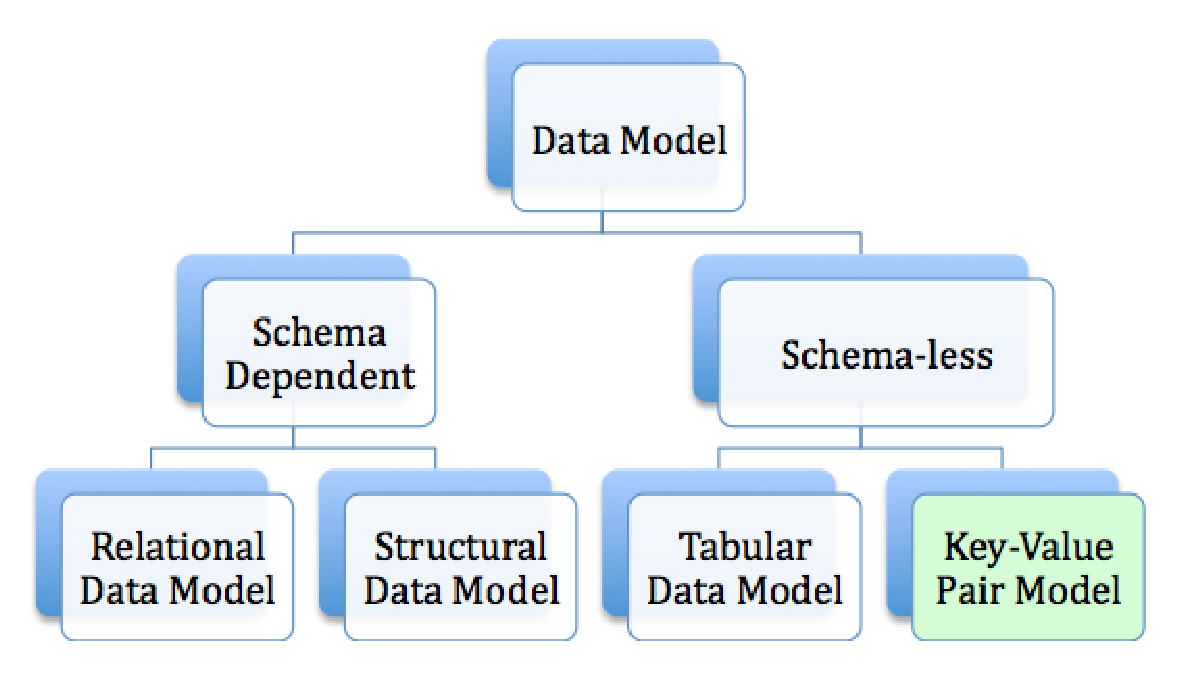
\includegraphics[scale=0.5]{../diagrams/taxonomy-data-model-modified}
  \caption{Data Model Taxonomy}
  \label{fig:taxonomy-data-model-modified}
\end{figure}

Another aspect of the implementation is that provides APIs in different
languages for the data creation and extraction processes. In this way, the
implementation of the persistence model captures the instances of any known
data collected from NetBEAMS and saves it using the document pattern as shown
in Listing \ref{file:mongodb-ysi-data-format}. One application of a
schema-less data model is the addition of any new key-value pair to any
instance of the document, as mongoDB supports update operations to any of the
collections. It can use tags for the purpose of annotations as described in the
taxonomy of data description. For example, in case of an oil spill in the San
Francisco Bay occurs, researchers can update the data set of a given date
range by adding tags to the relating documents. As a consequence of the use of
a schema-less data model, these changes do not affect the other data
instances, since there are no schema changes.

As described in chapter 5, the schema-less data model can provide a better
support to Data Provenance because the data model gives support to the change
of records without affecting the others. In this way, the metadata used by the
implementation clearly describes the three fundamental questions regarding the
collected data from sensor devices, as described in section
\ref{sec:keys-definition}. First, the identity of the data is given by the key
``message\underline{ }id'', in a way that it uniquely identifies the data
produced by the sensor identified by the key ``sensor.ip\underline{
}address''. In this way, the message can be tracked back to the sensor that
produced the data for different purposes such as tracking the data producer.
Second, time dimensions were used in order to track two different aspects of
the data collection: the valid time can be used to correlate observations to
the exact moment it occurred, while the transaction time can be used to verify
when the data was collected, and make decisions such as deleting the instances
of data were collected in the previous two days, etc. Last, but not least, the
use of the key ``sensor.location'' can give the exact location of the data,
since researchers can be interested in finding data based on a specific
location. Finally, the most important aspect of the schema-less data model is
that the observed data is added to the key ``observation'', as any sensor
device carries its set of attributes of key-value pairs. A good example of the
applicability of the schema-less data model is the scalability regarding
changes to the data structure. For instance, if an existing sensor device is
flushed with a new version of the firmware\footnote{The first set of machine
instructions to run on the hardware after the application of power stored
permanently in PROM or ROM or semi-permanently in EPROM}, changing the format
of data types or adding new values, the following instances of collected data
may be different to the previous one by simply adding the new additions of
data. For this reason, the DSP Data Persistence gives administrators the
ability to choose which fields to persist by declaring it using a bootstrap
message for the component, as shown in the parameter ``YSI\underline{
}DESIRED\underline{ }PROPERTIES'' of Listing
\ref{file:dsp-data-persistence-bootstrap.xml}.

The centralized query processing used by NetBEAMS is a result of the
infrastructure used by NetBEAMS, as well as the purpose of data and the
location of the collected data. As a direct result of a schema-less data
model, the centralized query processing is easily developed using any of the
available programming languages provided by mongoDB. Considering the fact that
programming languages are easier abstractions to researchers without computer
science background \cite{sn-programming-language}, mongoDB's approach to data
access through API can be seen as an easier task to manage data. As it is shown
in Listing \ref{file:experiment-query-scenarios}, the scenarios designed to
evaluate the implementation are written in Javascript, since it is the script
language by the mongoDB Shell. Therefore, it attends the requirement of not
using the SQL language as the main query language of the data, giving a better
data access abstraction similar to programming languages for different users.

One of the most important features of a data persistence for sensor
networks is the replacement of the SQL by the use of programming
languages, as they tend to be easier abstraction to users without the
background in database systems \cite{sn-programming-language}. In this way,
mongoDB covers the requirements of providing data access to the collected
sensor data in different languages. For example, the data collected by the DSP
Data Persistence component is written in Java, while the implementation of the
experiments scenarios for querying the collected data is given in Javascript. In
this way, researchers of the RTC may choose one of the enumarated languages
APIs provided by the mongoDB to access the stored data from NetBEAMS.

Finally, the implementation supported by mongoDB during the experiments was
following a single dedicated server virtualization using VirtualBox 
\cite{virtualization}.

\subsection{Infrastructure Evaluation}

Overall, the implementation of the DSP Data Persistence component meets
the specification of the use cases defined in section \ref{sec:exp-scenarios}.
The implementation of mongoDB using a single server environment can give
support to the current workload and infrastructure from the use of NetBEAMS to
collect data from the sensors devices from SF-BEAMS. From the perspective of
disk-space utilization and given that aproximaly 1.3 Gigabytes of disk space
were used to save one year-worth of collected data equivalent to five YSI
devices. According to the mongoDB documentation \ref{mongodb}, the claimed
amount of disk space is related to how mongoDB uses a binary representation
of the JSON documents, which are composed only of strings, together with the
definition of the indexes also represent in JSON. As a consequence, the size of
the keys defined for the YSI sonde data defines the amount of disk space used.
For this reason, different experiments were conducted with different
definitions of the keys of the documents
approach when compared the the RTC's OPEnDAP format shown in Listing
\ref{file:rtc-ysi-opendap}. Then, the second specification used short names
for the keys. In this way, the amount of storage space utilized by for the
different workloads define in section \ref{sec:workload} can be summarized as
follows

The performance to insert data into the database system using the Java driver
is documented by mongoDB as the fastest approach, providing persistence to
approximaly 25,091 documents per minute on an indexed database. In contrast,
when indexes are not used, more then 169,508 documents could be inserted per
minute. Although the latter approach supports more ducuments than the former,
the trade off between insertion and selection time is relevant due to the
activities of retrieval for documents for specific periods of time. Therefore,
the use of indexes might speed the retrieval time considerably. Considering
this number of insertions to the database the number of sensors producing data
and sending to the data sink, mongoDB and NetBEAMS implementation can
virtually support thousands sensor devices.

Disk utilization is one important characteristic of the selected database
system. However, the retrieval of the collected data from sensor devices is
a much more important requirement because most of the utilization of the data
persistence of a sensor network is regarding the search for the properties on
the collected data. After analyzing the response times for the scenarios
described in section \ref{sec:exp-scenarios}, it is clear that the use of
indexes improves the overall execution of the queries, specially because of the
amount of data collected over the years. Furthermore, the response times
described in this scenario is directly related to the use of the External
Storage strategy. On the other hand, improvements over the response time can be
achieved through the implementation of a Data-Centric approach on a Distributed
Database environment, or clusters. In this approach, the inserted data is
stored in different servers based on a partition key. Given the fact that less
data is concentrated in each partition, the centralized query mechanism used is
faster, and consequently improves the performance as described in the Data
Location taxonomy in chapter 3.

When it comes to re-using the data collected by the DSP Data Persistence,
different approaches were available. First, the use of the export capabilities
to a common-delimited values was performed \ref{file:mongodb-export-command},
taking approximaly 3.3 minutes to export one year worth of data for 5 YSI
devices without indexing. Second, the use of the client shell gives a
centralized access to either the single server. However, in order to better
provide access of data to users without skills in database systems, web
applications can be built on top of the REST Web Services APIs \cite{http-rest}
provided by mongoDB. One such example of using the REST API is the adaptation
of Apache Futon 4 mongoDB, as shown in Figure
\ref{fig:view-collections-instance-browser-futondb}, where users can navigate
through the collections of the collected sensor network data categorized by the
collection. Therefore, RTC staff technicians could take advantage of this tool
to view and navigate over the collected data from the sensor devices.

\subsection{Use Cases Evaluation}

Supposing an environmental accident such as the San Francisco oil
  spill happened again \cite{sfbay-oilspill2009}, changing the sampling
  frequency drastically to different values. 

\section{Difficulties Experienced}
\label{sec:experiments-difficulties}
As the development of computing system, the inception of the experiments
described in this chapter had different moments of Software Engineering.
Particularly speaking about the learning curve, different situations
contributed to the success of the first experiments. Since the technoogy is
new, it brought new challenges regarding the usability and user experience.
Since the technology is relatively new and still under development, many
different bugs were could be reproduced by random during the execution of the
experiments, and therefore, sent to the open-source community through use 
different available communication channels. First, the fastest way to solve an
issue was through the mongoDB's IRC channel, located at the Freenode server
(www.freenode.org, channel mongodb). Second, the use of the users group, located
at http://groups.google.com/group/mongodb-user also helped solving problems.

Physical memory is limited, for this reason, it may not be enough to run the
experiments for total workloads. In this case, the Java Virtual Memory was
totally consumed by one of the revisions of the experiments setup. Huge data
loads require different approach to manage data in memory such as creating
object pools as temporary cache for objects whose state are similar to others.

While performing the experiments, the 32bit machine reached its limitation of
2GB of physical data. With know about that, the environment needed to be
updagred for mongoDB requires a 64-bit operating system when the amount of
stored data reaches 2 Gigabytes. For this reason, the scenarios with indexes
used a dedicated virtualized server using Ubuntu Linux 9.04 64 bits with 1 Gb
of memory.